\documentclass[output=paper,
colorlinks,
citecolor=brown,
newtxmath
]{langscibook}
\bibliography{localbibliography}

\author{Olav Mueller-Reichau\affiliation{Leipzig University}}
\title{Perfective \textit{dozapisyvat'} -- real or fake?}
\abstract{
The paper discusses perfective verbs like \textit{dozapisyvat'} or \textit{dovyšivat'} in which, contrary to what current theories of Russian verb formation would have predicted, a positionally restricted prefix attaches above secondary imperfective morphology. In the first part of the paper it is shown that the phenomenon is real, and should not be denied or ignored. In the second part it is argued that the otherwise observed prohibition of positionally restricted prefixes over secondary imperfective suffixes is a case of pragmatic blocking. It is proposed that perfective verbs like \textit{dozapisyvat'} are possible because in the specific case of \textit{do-} the morphological blocking mechanism may be suspended under certain contextual circumstances, i.e. when reference is made to the final element within a sequence of completed events describable by the verb without this prefix.

\keywords{Russian, verb formation, aspect, imperfectivizing suffix, positionally restricted prefix, iterativity, morphological blocking}
}

% add all extra packages you need to load to this file

\usepackage{tabularx,multicol}
\usepackage{url}
\urlstyle{same}

\usepackage{listings}
\lstset{basicstyle=\ttfamily,tabsize=2,breaklines=true}

\usepackage{langsci-optional}
\usepackage{langsci-lgr}
\usepackage{langsci-gb4e}
\usepackage[linguistics]{forest}
\usepackage{setspace}
\usepackage{pifont}
\usepackage[normalem]{ulem}
\usepackage{tabto}

\usepackage{relsize}


\usepackage{multicol}
\usepackage{textgreek}

\newcommand*{\orcid}{}


% \IfFileExists{../localcommands.tex}{%hack to check whether this is being compiled as part of a collection or standalone
%   % add all extra packages you need to load to this file

\usepackage{tabularx,multicol}
\usepackage{url}
\urlstyle{same}

\usepackage{listings}
\lstset{basicstyle=\ttfamily,tabsize=2,breaklines=true}

\usepackage{langsci-optional}
\usepackage{langsci-lgr}
\usepackage{langsci-gb4e}
\usepackage[linguistics]{forest}
\usepackage{setspace}
\usepackage{pifont}
\usepackage[normalem]{ulem}
\usepackage{tabto}

\usepackage{relsize}


\usepackage{multicol}
\usepackage{textgreek}

%   \newcommand*{\orcid}{}

\togglepaper[11]
% }{}

\begin{document}
\shorttitlerunninghead{Perfective \textup{dozapisyvat'} -- real or fake?}
\maketitle

%%%%%%%%%%%%%%%%%%%%%%%%%%%%%%%%%%%%%%%%%%%%%%%%%%%%%%%%%
% Section 1
%%%%%%%%%%%%%%%%%%%%%%%%%%%%%%%%%%%%%%%%%%%%%%%%%%%%%%%%%

\section{Introduction}

The present paper contributes to a recent debate concerning the structure of the Russian verb. It addresses the question of whether the prefix \textit{do-} in its ``completive'' usage may attach to a verbal base which already contains secondary imperfective morphology, giving rise to perfective forms like the one in the title of this article.

The background of the matter is the fine-grained analysis of Russian verbal morphology outlined in \citet{Tatevosov2009} and \citet{Tatevosov2013b}. In these two articles, the author presents a detailed inventory of the Russian prefixes, which supersedes the well-known bipartition into internal/lexical and external/super\-lexical pre\-fixes (see \citealt{Gehrke2008}; \citealt{Ramchand2004}; \citealt{Romanova2004}; \citealt{Svenonius2004}; among others). Relevant for the present paper is the proposed class of so-called \textsc{positionally restricted} (PR-)prefixes, which has at least the three members noted below (see \citealt[49]{Tatevosov2013b}):

\ea\label{tatprefs}
\begin{itemize}
\item[] external prefixes
    \begin{itemize}
    \item[] left-peripheral prefixes
        \begin{itemize}
        \item[] \textit{po-}\textsuperscript{distributive}
        \end{itemize}
    \item[] selectionally restricted prefixes
        \begin{itemize}
        \item[] \textit{za-}\textsuperscript{inchoative}
        \item[] \textit{po-}\textsuperscript{delimitative}
        \item[] {\dots}
        \end{itemize}
    \item[] positionally restricted prefixes
        \begin{itemize}
        \item[] \textit{do-}\textsuperscript{completive}
        \item[] \textit{pere-}\textsuperscript{repetitive}
        \item[] \textit{pod-}\textsuperscript{attenuative}
        \end{itemize}
\end{itemize}
\item[] internal prefixes
        \begin{itemize}
        \item[]
            \begin{itemize}
            \item[] \textit{u-}
            \item[] \textit{-v}(\textit{o})\textit{-}
            \item[] \textit{nad}(\textit{o})\textit{-}
            \item[] {\dots}
            \end{itemize}
        \end{itemize}
\end{itemize}
\z

\noindent According to Tatevosov, PR-prefixes are free to apply to perfective or imperfective bases, but are fixed to a structural position lower than the secondary imperfective morpheme \textit{yv(a)}. Thus, Tatevosov's theory entails the following generalization:

\ea\label{tategen}
Generalization [$\text{*PR}>\text{\textit{yva}}$]\\
Positionally restricted (external) prefixes must not apply above secondary imperfective morphology (\textit{yva}).
\z

\noindent Now \citet{Zinova.Filip2015} and in particular \citet{Zinova2016} have drawn attention to a class of verbs representing counterevidence to \REF{tategen}. Their paradigmatic examples are \textit{dozapisyvat'} `finish recording' and \textit{dovyšivat'} `finish embroidering'. According to \citet{Zinova.Filip2015}, these verbs are perfective when derived along the derivational histories in \REF{dh1}:

\ea\label{dh1}
\ea \textit{pisat'}\textsuperscript{\textsc{ipfv}} $\rightarrow$ \textit{zapisat'}\textsuperscript{\textsc{pfv}} $\rightarrow$ \textit{zapisyvat'}\textsuperscript{\textsc{ipfv}} $\rightarrow$ \textit{dozapisyvat'}\textsuperscript{\textsc{pfv}}
\ex \textit{šit'}\textsuperscript{\textsc{ipfv}} $\rightarrow$ \textit{vyšit'}\textsuperscript{\textsc{pfv}} $\rightarrow$ \textit{vyšivat'}\textsuperscript{\textsc{ipfv}} $\rightarrow$ \textit{dovyšivat'}\textsuperscript{\textsc{pfv}}
\z\z

\noindent If these assumptions are correct, \textit{do-}\textsuperscript{completive} applies to a secondarily imperfectivized form in these cases, thus falsifying [$\text{*PR}>\text{\textit{yva}}$].
The aim of this paper is to assess this conclusion by asking the following two questions.

\begin{exe}
\ex\label{2questions}
\begin{xlist}
\exi{[Q1]}{Is there really a perfective verb \textit{dozapisyvat'}?}
\exi{[Q2]}{If yes, does it really falsify Tatevosov's theory?}
\end{xlist}
\end{exe}

\noindent Jumping ahead, I will answer the first question affirmatively and the second one negatively. There is something special about \textit{do-} that makes it a systematic exception to the otherwise valid generalization \REF{tategen}.

The paper is structured as follows. In \sectref{sec2} I introduce the phenomenon: verbs like \textit{dozapisyvat'} that allow for an expected imperfective, but also for an unexpected perfective reading. \sectref{H1} points to four issues related to these verbs that until now have either not been asked or not been answered. Before introducing my own proposal, \sectref{sec4} is inserted to demonstrate the weaknesses of alternative explanations of the phenomenon that might come to mind. In \sectref{prop} I outline my own analysis. I show that the prefix \textit{do-} may attach to a base involving secondary imperfective morphology only if the base denotes a plurality of successively realizing completed events.
I will explain why this is so and how this accounts for the open issues addressed in \sectref{H1}.
\sectref{concl} concludes the paper.

%%%%%%%%%%%%%%%%%%%%%%%%%%%%%%%%%%%%%%%%%%%%%%%%%%%%%%%%%
% Section 2
%%%%%%%%%%%%%%%%%%%%%%%%%%%%%%%%%%%%%%%%%%%%%%%%%%%%%%%%%

\section{The biaspectual behavior of \textit{dozapisyvat'}}\label{sec2}

Let me briefly recapitulate the properties of the class of verbs identified by \citet{Zinova.Filip2015}. Following the authors' practise, I will use the verbs noted above as representatives of the whole class.

To begin with, \textit{dozapisyvat'} and \textit{dovyšivat'} are capable of expressing imperfective meanings:

\ea\label{songpfin1}
\gll Ja dozapisyvaju pesnju uže 2 časa.\\
I {finish.record.}\textsc{prs.ipfv} song already 2 hours\\
\glt `I am finishing recording the song already for 2 hours.' \hfill \citep[16]{Zinova2016}
\z

\ea\label{songipf2}
\gll Vot v dannyj moment dozapisyvaju {Alan Wake}.\\
 \textsc{prt} in given moment {finish.record.}\textsc{prs.ipfv} A.W.\\
\glt `At the very present moment I am finishing recording Alan Wake.'\footnote{``Alan Wake'' is a video game.}  \\ \hfill (\url{www.x360-club.org/forum})
\z

\ea\label{kotiki}
\gll Chorošen'kie! A ja {kak raz} dovyšivaju kotiki!!! Skoro pokažu!\\
 cute but I now {finish.embroider.}\textsc{prs.ipfv} tomcats
 soon show-\textsc{prs.pfv}\\
\glt `How cute! And I am right now finishing embroidering the tomcats!!! I will show them soon.' \hfill (\url{www.chudokrestik.forum2x2.ru})
\z

\noindent As examples \REF{songpfin1} to \REF{kotiki} show, the relevant verbs may clearly be used as imperfectives. This does not come as a surprise. Apart from that usage, however, \textit{dozapisyvat'} and \textit{dovyšivat'} can arguably also express perfective meanings. The first evidence for this conclusion stems from compatibility with inclusive time adverbials. As shown in \citet[16]{Zinova2016}, such adverbials are strictly ruled out for verbs like \textit{dopisyvat'} \REF{sss} but possible with with verbs like \textit{dozapisyvat'} \REF{songpfin2} and \textit{dovyšivat'} \REF{songpfin3}.

\ea[*]{\gll Ja dopisyvaju pesnju za 2 časa.\\
I {finish.write.}\textsc{prs.ipfv} song within 2 hours\\
\glt Intended: `I will finish writing the song in 2 hours.'\label{sss}}
\z

\ea\label{songpfin2}
\gll Ja dozapisyvaju pesnju za 2 časa.\\
I {finish.record.}\textsc{prs.pfv} song within 2 hours\\
\trans `I will finish recording the song in 2 hours.'
\z

\ea\label{songpfin3}
\gll Ja dovyšivaju kartinu za 2 časa.\\
I {finish.embroider.}\textsc{prs.pfv} picture within 2 hours\\
\glt `I will finish embroidering the picture in 2 hours.'
\z

\noindent Another indication of perfectivity is that verbs like \textit{dozapisyvat'} can move the reference time forward in narratives.

\ea\label{songpfnarr1}
\gll Ja dozapisyvaju disk i pojdu domoj.\\
I {finish.record.}\textsc{prs.pfv} CD and go.\textsc{prs.pfv} home\\
\glt `I will finish recording the CD and go home.' \hfill \citep[32]{Zinova2016}
\z

\noindent The significance of this test is emphasized by the fact that a verb like \textit{dopisyvat'} `finish writing', which has external \textit{do-} but no internal prefix, does not support narrative progression.

\ea[*]{\label{tekstpfnarr1}
\gll Ja dopisyvaju tekst i pojdu domoj.\\
I {finish.write.}\textsc{prs.ipfv} text and go.\textsc{prs.pfv} home\\
\glt Intended: `I will finish writing the text and go home.' \hfill \citep[32]{Zinova2016}}
\z

\noindent The same pattern can be observed with respect to \textit{dovyšivat'} and \textit{došivat'} `finish sewing':

\ea\label{kartpfnarr0}
\gll Ja dovyšivaju kartinu i pojdu domoj.\\
I {finish.embroider.}\textsc{prs.pfv} picture and go.\textsc{prs.pfv} home\\
\glt `I will finish embroidering the picture and go home.'
\z

\ea[*]{\label{kartpfnarr1}
\gll Ja došivaju plat'e i pojdu domoj.\\
I {finish.sew.}\textsc{prs.ipfv} dress and go.\textsc{prs.pfv} home\\
\trans Intended: `I will finish sewing the dress and go home.'}
\z

\noindent \REF{mono} is an authentic example to show, once more, that \textit{dovyšivat'} with present tense inflection (here: 1st person singular) can be used under future reference without further ado -- as is characteristic of a perfective verb.\footnote{``Without further ado'' is added here because also imperfective verbs may have future reference, but only if accompanied by expressions such as \textit{zavtra} `tomorrow' in \textit{Zavtra ja idu v kino} `Tomorrow I go to the cinema'. No such expression is present in \REF{mono}. Thanks to an anonymous reviewer for pointing that out.}

\ea\label{mono}
\gll Kartina, za kotoruju ja vzjalas', monochromnaja, skučnovato ee vyšivat' okazalos', no ja ee dovyšivaju objazatel'no! \\
picture behind \textsc{pron} I {attend.to.}\textsc{pst.pfv} monochrome
boring her embroider.\textsc{inf.ipfv} {turn.out.}\textsc{pst.pfv}
but I her {finish.embroider.}\textsc{prs.pfv} unconditionally\\
\trans `The picture that I attended to is monochrome, embroidering it turned out to be boring, but I will definitely finish embroidering it.'\\ \hfill (\url{www.stranamasterov.ru/})
\z

\noindent From observations like those presented above, \citet{Zinova.Filip2015} conclude that verbs like \textit{dozapisyvat'} come in two versions, one perfective and one imperfective, related to two different derivational histories \REF{2hist}. The version \REF{2histb} falsifies Tatevosov's generalization [$\text{*PR}>\text{\textit{yva}}$]:

\ea\label{2hist}
\ea {[}[do-[za-[pis-]\textsuperscript{\textsc{ipfv}}]\textsuperscript{\textsc{pfv}}]\textsuperscript{\textsc{pfv}}yva-]\textsuperscript{\textsc{ipfv}} \label{2hista}
\ex {[}do-[[za-[pis-]\textsuperscript{\textsc{ipfv}}]\textsuperscript{\textsc{pfv}}yva-]\textsuperscript{\textsc{ipfv}}]\textsuperscript{\textsc{pfv}} \label{2histb}
\z\z

%%%%%%%%%%%%%%%%%%%%%%%%%%%%%%%%%%%%%%%%%%%%%%%%%%%
% Section 3
%%%%%%%%%%%%%%%%%%%%%%%%%%%%%%%%%%%%%%%%%%%%%%%%%%%

\section{Four open questions}\label{H1}

We saw that, according to \citet{Zinova.Filip2015} and \citet{Zinova2016}, verbs such as \textit{dozapisyvat'} and \textit{dovyšivat'} may express not only imperfective, but also perfective meanings. The perfective verb \textit{dozapisyvat'} derives from prefixing the imperfective \textit{zapisyvat'} with \textit{do-} in completive function. This violates the constraint [$\text{*PR}>\text{\textit{yva}}$], thus falsifying \citeposst{Tatevosov2013b} theory. Straightforward as this conclusion is, a number of issues arises from this proposal. There are at least four open questions.

%%%%%%%%%%%%%%
% Section 3.1
%%%%%%%%%%%%%%

\subsection{No blocking?}

Why is perfective \textit{dozapisyvat'} not blocked by the availability of perfective \textit{dozapisat'}? Wouldn't we expect the pragmatic principle `avoid complexity of expression' \citep{Kiparsky2005}, here stated in the version of \citet{LeBruyn2007}, to rule out the morphologically more complex perfective verb \textit{dozapisyvat'}?

\ea\label{avoid} Avoid complexity principle\\All other things being equal, less complex expressions are preferred over more complex expressions.
\z

\noindent Take \REF{songpfnarr1} from above, for instance. Why is the possibility of perfective \textit{dozapisyvaju} not blocked by the existence of perfective \textit{dozapišu}? The constructed example \REF{block1} makes the same point, involving a different verb: why is perfective \textit{doustanavlivaju}, which is acceptable in this context, not blocked by perfective \textit{doustanovlju}?\footnote{\label{f1}Some of my informants have stylistic concerns about \textit{doustanavlivat'}.}

\ea\label{block1}
\gll Ja doustanavlivaju Windows i pojdu domoj.\\
I {finish.install.}\textsc{prs.pfv} W. and go.\textsc{prs.pfv} home\\
\glt `I will finish installing Windows and go home.'
\z

%%%%%%%%%%%%%%
% Section 3.2
%%%%%%%%%%%%%%

\subsection{Constraints on coordination order?}\label{arte}

Next, consider the following two examples.

    \largerpage[-1] % to move ex. (20) to next page

\ea\label{machanik}
\gll Mechanik dozapravljal samolet i zakuril sigaretu.\\
mechanic {finish.fill.}\textsc{pst.pfv} plane and {start.smoke.}\textsc{pst.pfv} cigarette\\
\glt `The mechanic finished fueling the plane and lightened a cigarette.' \\ \hfill \citep[175]{Zinova2016}
\z

\ea[??]{
\gll Mechanik zakuril sigaretu i dozapravljal samolet.\\
mechanic {start.smoke.}\textsc{pst.pfv} cigarette and {finish.fuel.}\textsc{pst.pfv} plane\\
\glt Intended: `The mechanic lightened a cigarette and finished fueling the plane.'\label{macha}}
\z

\noindent It can be observed that \REF{macha} is worse than \REF{machanik}. But why should that be so? Given that the form \textit{dozapravljal} may serve as a perfective verb, as \citet{Zinova.Filip2015} and \citet{Zinova2016} suggest, there is no \textit{prima facie} reason why switching the elements of the event chain in \REF{machanik} should lower acceptability. Note that if we replace \textit{dozapravljal} by its perfective rival \textit{dozapravil}, the discourse will be sound again.

\ea\label{machaplus}
\gll Mechanik zakuril sigaretu i dozapravil samolet.\\
mechanic {start.smoke.}\textsc{pst.pfv} cigarette and {finish.fuel.}\textsc{pst.pfv} plane\\
\glt `The mechanic lightened a cigarette and finished fueling the plane.'
\z

%%%%%%%%%%%%%%
% Section 3.3
%%%%%%%%%%%%%%

\subsection{What about other PR-prefixes?}\label{popopo}

How do we explain that \textit{do-} seems to be the only PR-prefix that can perfectivize secondary imperfectives? Indeed, \textit{pere-} in repetitive function as well as \textit{pod-} in attenuative function do not seem to allow for this option:

\ea[*]{\label{songpfnarrz}
\gll Ja perezapisyvaju disk i pojdu domoj.\\
I {again.record.}\textsc{prs.pfv} disc and go.\textsc{prs.pfv} home\\
\glt Intended: `I will record the disc again and go home.'}
\z

\ea[*]{\label{podza}
\gll Ja podzarabatyvaju den'gi i pojdu domoj.\\
I {a.bit.earn.}\textsc{prs.pfv} money and go.\textsc{prs.pfv} home\\
\glt Intended: `I will earn a little money and go home.'}
\z

\noindent \citet{Zinova.Filip2015} are well aware of the fact that the form \textit{perezapisyvat'} is always imperfective. They conclude that \textit{pere-}, unlike \textit{do-}, yields an imperfective verb when built along a derivational chain analogous to \REF{2histb}, and call this an ``intriguing exception to the general pattern according to which the output of prefixation is perfective'' \citep[605]{Zinova.Filip2015}. If correct, that would indeed be an ``intriguing exception'' because it would run against common wisdom in Russian aspectology:

\begin{quote}
    V sovremennom russkom jazyke dejstvuet sledujuščij zakon: ljuboj glagol, polučennyj prisoedineniem pristavki k nekotoromu drugomu glagolu (i ne podvergšijsja dal'nejšej imperfektivacii), javljaetsja glagolom sov. vida.\\ \null\hfill\citep[67]{Zaliznjak.Smelev1997}\smallskip\\
    $[$In modern Russian there is the following law: any verb resulting from the attachment of a prefix to some other verb (and which is not subjected to further imperfectivization thereafter) is a perfective verb.$]$
\end{quote}

%%%%%%%%%%%%%%
% Section 3.4
%%%%%%%%%%%%%%

\subsection{What makes a good example?}

Why are some forms instantiating the pattern do$+$\textsc{pref}$+$\textsc{root}$+$yva$+$t' much better as perfectives than others? Perfective \textit{dovyšivat'} is accepted by almost any speaker of Russian; perfective \textit{dozapisyvat'} is accepted by many, though by far not by all
\citep[see][16--17]{Zinova2016}.

Thus \REF{Zin6} and \REF{ustanav} are fine for every native speaker of Russian I consulted, whereas \REF{Zin5} raises disagreement.\footnote{\label{f2}But see fn. \ref{f1}.} What is missing is an explanation of this asymmetry in acceptability within the respective class of verbs.

\ea\label{Zin6}
\gll Ja dovyšiyvaju kartinu i pojdu domoj.\\
I {finish.embroider.}\textsc{prs.pfv} picture and go.\textsc{prs.pfv} home\\
\glt `I will finish embroidering the picture and go home.'
\z

\ea\label{ustanav}
\gll Ja doustanavlivaju Windows i pojdu domoj.\\
I {finish.install.}\textsc{prs.pfv} W. and go.\textsc{prs.pfv} home\\
\glt `I will finish installing Windows and go home.'
\z

\ea\label{Zin5}
\gll Ja dozapisyvaju pesnju i pojdu domoj.\\
I {finish.record.}\textsc{prs.pfv} song and go.\textsc{prs.pfv} home\\
\glt `I will finish recording the song and go home.'
\z

\noindent In this section, I have pointed to four questions that await being answered given the way \citet{Zinova.Filip2015} analyze the biaspectual behavior of verbs like \textit{dozapisyvat'}.
In the next section, I will pursue possible alternative treatments of the phenomenon.

%%%%%%%%%%%%%%%%%%%%%%%%%%%%%%%%%%%%%%%%%%%%%%%%%%%%%%%%
% Section 4(.1)
%%%%%%%%%%%%%%%%%%%%%%%%%%%%%%%%%%%%%%%%%%%%%%%%%%%%%%%

\section{Exploring alternative explanations}\label{sec4}

\subsection{Fake perfectives}\label{H2}

This subsection addresses question [Q1] in \REF{2questions} by checking for the possibility that the perfectivity of \textit{dozapisyvat'} (and its counterparts) is actually a mirage.

In view of the empirical evidence presented above, isn't it totally absurd to raise such a hypothesis? Maybe yes, but note that imperfective coding does not \textit{per se} rule out a verb from the first sentence in a chain-of-events, i.e. from a discourse where the event denoted by the first sentence is related to the event of the second sentence via narration \citep[31]{Zinova2016}. The prerequisite for this possibility is that the second sentence is introduced by the connective \textit{potom} `then':

\ea\label{eis1}
\gll Ja zavtrakaju, potom pojdu na rabotu.\\
I {have.breakfast.}\textsc{prs.ipfv} then go.\textsc{prs.pfv} on work\\
\glt `I am eating breakfast, afterwards I will go to work.'
\z

\noindent With respect to \textit{dozapisyvat'}, the idea would be that \textit{do-}
explicitly marks the first event in (\ref{doipf}) as finalizing a discourse constituent (inviting the inference of an implicit \textit{potom}, so to speak), just like explicit \textit{potom} marks the second event in (\ref{eis1}) as starting a new discourse constituent.

\ea\label{doipf}
\gll Ja dozapisyvaju disk i pojdu domoj.\\
I {finish.record.}\textsc{prs.ipfv} disc and go.\textsc{prs.pfv} home\\
\glt`I am finishing recording the disc, afterwards I will go home.'
\z

\noindent A story along these lines could explain why the PR-prefixes \textit{pere-} and \textit{pod-} are not capable of forming perfective verbs when attaching to \textit{zapisyvat'} or \textit{vyšivat'}. But it cannot explain why \REF{naeh} is bad:

\ea[*]{\label{naeh}
\gll Ja došivaju plat'e i pojdu domoj.\\
I {finish.sew.}\textsc{prs.ipfv} dress and go.\textsc{prs.pfv} home\\
\glt Intended: `I am finishing sewing the dress, afterwards I will go home.'}
\z

\noindent An argument in favor of the hypothesis that \textit{dozapisyvat'} is always imperfective might be drawn from the observation that \REF{noplusqu} displays no pluperfect reading.\footnote{The sentences \REF{noplusqu} to \REF{noplusqu2} all allow for an imperfective interpretation according to which the agent of the subordinate clause came when Ivan was already engaged in finishing recording the discs, embroidering the picture, or installing Windows.}

\ea\label{noplusqu}
\gll Kogda načal'nik prišel k Ivanu, tot uže dozapisyval trebuemye diski.\\
when boss come.\textsc{pst.pfv} to I. \textsc{dem} already {finish.record.}\textsc{pst.pfv} demanded discs\\
\glt Not: `When the boss came to Ivan, he (Ivan) had already finished recording the demanded discs.'
\z

\noindent But maybe in this case the perfective construal of \textit{dozapisyval} is blocked by \textit{dozapisal}. Indeed, with \textit{dovyšivat'}, for which there is no shorter perfective alternative (the form *\textit{dovyšit'} does not exist in Russian), the pluperfect reading seems available:

\ea\label{yesplusqu}
\gll Kogda ja prišel k Ivanu, tot uže dovyšival kartinu.\\
when I come.\textsc{pst.pfv} to I. \textsc{dem} already
{finish.embroider.}\textsc{pst.pfv} picture\\
\glt Possible: `When I came to Ivan, he (Ivan) had already finished embroidering the picture.'
\z

\noindent Now note that also for \textit{doustanavlivat'}, which does have a morphologically simpler perfective correlate in \textit{doustanovit'},
the pluperfect reading is available. Concluding from \REF{noplusqu} that \textit{dozapisyvat'} cannot be perfective is thus premature.

\ea\label{noplusqu2}
\gll Kogda ja prišel k Ivanu, tot uže doustanavlival Windows.\\
when I come.\textsc{pst.pfv} to I. \textsc{dem} already {finish.install.}\textsc{pst.pfv} W.\\
\glt Possible: `When I came to Ivan, he (Ivan) had already finished installing Windows.'
\z

\noindent In view of the facts discussed in this section, the idea that the perfective behavior of verbs like \textit{dozapisyvat'}, \textit{dovyšiyvat'},  \textit{doustanavlivat'}, etc. could be only apparent must be abandoned. Perfective \textit{dozapisyvat'} is real.

%%%%%%%%%%%%%%
% Section 4.2
%%%%%%%%%%%%%%

\subsection{Internal iterative \textit{yva}}\label{H3}

Now I will pursue the hypothesis that there really is a perfective version of \textit{dozapisyvat'}, but that in this version the suffix \textit{yv(a)} is no secondary imperfective morpheme, but rather an iterativizer. There are two ways in which this idea may be implemented: suffixation may take place before or after prefixation. The second option will be addressed in \sectref{H4}. According to the first option, where \textit{yv(a)} attaches low, suffixation serves to form an iterative stem from a simple root, i.e. \textit{pisyv(at')} from \textit{pis(at')} \citep[see][]{Paduceva2015}. When a lexical/internal prefix (here: \textit{za-}) applies to such an iterative base (here: \textit{pisyva-}), it will modify the event kind that is claimed to be realized repeatedly. In the given case this will lead from denoting multiple realizations of writing events to denoting multiple realizations of recording events. As for the external prefix \textit{do-}, we assume, for the sake of the argument, that when stacking on top, it induces an upper closed ``temporal macro event scale'', as indicated in \figref{fig:macroscale} (more on that below). The natural numbers indicate the number of events (in our case: recording events) that have occurred up to the respective point of time on the scale. The scale is upper-closed in that there is one point that demarcates the maximal number of events. In \figref{fig:macroscale} the maximal number of events is arbitrarily chosen as ten. Note further that the ten recording events symbolized in \figref{fig:macroscale} are ten maximal/completed recording events (the prefix \textit{za-} introduces the respective maximality condition; see \sectref{H51}).

\begin{figure}
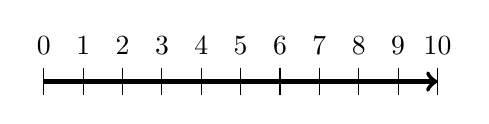
\begin{tikzpicture}
  \foreach \x in {0,1,2,...,10}
    {
      \coordinate (A\x) at ($(0,0)+(\x*0.5cm,0)$) {};
      \draw ($(A\x)+(0,5pt)$) -- ($(A\x)-(0,5pt)$);
      \node at ($(A\x)+(0,3ex)$) {\x};
    }
  \draw[ultra thick,arrows=->] (A0) -- (A10);
\end{tikzpicture}
\caption{Upper closed macro event scale}
\label{fig:macroscale}
\end{figure}

Let us assume further that, unlike \textit{do-}\textsuperscript{completive}, the prefixes \textit{pere-}\textsuperscript{repetitive} and \textit{pod-}\textsuperscript{attenuative} do not have the capacity of ordering the plurality of events in its input on a macro scale like \figref{fig:macroscale}.

According to the story just sketched, the suffix \textit{yv(a)} in perfective \textit{dozapisyvat'} applies prior to the internal prefix \textit{za-}, i.e. itself VP-internally. It is thus a different creature than the secondary imperfective \textit{yv(a)} that figures in the constraint that Tatevosov identifies for PR-prefixes, which I repeat from above, this time in a direct quote from \citet[4]{Tatevosov2013b}:

% Example 34

\eanoraggedright {[$\text{*PR}>\text{\textit{yva}}$]}\\Pozicionno-ograničennye prefiksy prisoedinjajutsja ne vyše, čem pokazatel' vtoričnogo imperfektiva \textit{-yva-}.\smallskip\\
$[$Positionally restricted prefixes do not attach higher than the marker of secondary imperfectives \textit{yva}.$]$
\z

\noindent Since Tatevosov's restriction [$\text{*PR}>\text{\textit{yva}}$] is explicitly connected to the marking of secondary imperfectives, it would not be violated if the story just told was correct. But can it be correct?

If \textit{yv(a)} was a marker of iterativity in perfective \textit{dozapisyvat'}, \textit{dovyšivat'}, etc., the macroevent relative to which the prefix \textit{do-} ``picks out'' the terminative interval should be made of a plurality of completed recording events, embroidering events, etc. More generally put: For a form instantiating \textit{do}$+$\textsc{pref}$+$\textsc{root}$+$\textit{yva}$+$\textit{t'} to be acceptable as perfective, the events denoted by \textsc{pref}$+$\textsc{root}$+$\textit{yva} should be conceivable as consisting of a plurality of completed  \textsc{pref}$+$\textsc{root}-events, realizing one after the other. Provisionally I call this condition ``seriality requirement''.

The seriality requirement might point to an answer to the question of why some instances of \textit{do}$+$\textsc{pref}$+$\textsc{root}$+$\textit{yva}$+$\textit{t'}, such as \textit{dovyšivat'}, are widely accepted as perfectives in the tested sentences, while others such as \textit{dozapisyvat'} are not (recall \sectref{H1}). Note that the event denoted by \textit{vyšivat' kartinu} is easily conceivable as a series of by themselves completed embroidering events. Imagine I want to embroider the picture of a farm. First I embroider the sheep shelter, then I embroider the cock standing on dunghill, etc. Similar with the event denoted by \textit{ustanavlivat' Windows}, because installing a computer program typically consists of installing different subprograms (files) one by one. Our world knowledge about these kinds of events is thus in harmony with the requirement of a series of completed events. Not so for the event denoted by \textit{zapisyvat' pesnju}. This event is typically realized in one go. Otherwise the song would be interrupted and, so to speak, destroyed, undermining the very goal of the action. That we expect a song to be recorded in one go is at odds with the seriality requirement, which calls for a plurality of completed recordings, and this might be the reason why many informants reject \REF{Zin5}, but not \REF{ustanav} and \REF{Zin6}. An interesting observation in that regard is that judgements improve once \REF{Zin5} is framed in a music studio context. This fits into the picture because when a song is recorded in a music studio, different sound files will be recorded in a serial manner, one by one, each a completed recording, to make up the whole song in the end: first the trumpets get recorded, then the drums, etc.

And so, we hypothesized that it might be an obstacle for accepting a perfective verb instantiating the schema \textit{do}$+$\textsc{pref}$+$\textsc{root}$+$\textit{yva} if the \textsc{pref}$+$\textsc{root}$+$\textit{yva}-event cannot easily be conceived of as a series of completed subevents. So far, so good. Unfortunately, however, the idea of internal iterative \textit{yv(a)} faces severe problems.

First, it should be noted that this story involves a violation of the otherwise valid rule that the output of prefixation is perfective (recall \sectref{popopo}). The violation concerns the second step in the assumed derivational history:

\ea\label{dhx}
\textit{pisat'}\textsuperscript{\textsc{ipfv}} `write' $\rightarrow$ \textit{pisyvat'}\textsuperscript{\textsc{ipfv}}  `write again and again' $\rightarrow$ \textit{zapisyvat'}\textsuperscript{\textsc{ipfv}} `record again and again' $\rightarrow$ \textit{dozapisyvat'}\textsuperscript{\textsc{pfv}} `finish recording'
\z

\noindent A further concern is that the derivational history in \REF{dhx} gives rise to a bracketing paradox. The syntactic derivation is not in line with the subsequent steps of semantic composition as shown in \figref{fig:paradox}.

\begin{figure}
\begin{forest}
for tree={s sep=1cm, inner sep=0, l=0}
[\textit{zapisyv(a)-}
    [{\textit{za-}} ]
        [\textit{pisyv(a)-}
            [{\textit{-yv}} ]
                [\textit{pis(a)-}
                ]
        ]
    ]
]
\end{forest}\hspace{2cm}
\begin{forest}
for tree={s sep=1cm, inner sep=0, l=0}
[{\sib{zapisyv(a)-}}
    [{\sib{-yv}} ]
        [{\sib{zapis(a)-}}
    [{\sib{za-}} ]
    [{\sib{pis(a)-}} ]
    ]
]
\end{forest}
\caption{Bracketing paradox arising from \REF{dhx}}
\label{fig:paradox}
\end{figure}

The internal prefix \textit{za-}, which enters the syntactic derivation only after application of iterative \textit{yv(a)}, should have semantic access to the event description supplied by the initial predicate \textit{pisat'}\textsuperscript{\textsc{ipfv}}. This technical problem is perhaps not insurmountable; however, it is difficult to come up with an easy solution.

A further point relates to the particular case of perfective \textit{doustanavlivat'}. The problem is that there is no verb \textit{stanavlivat'} in Russian. The proposed derivational history would thus involve a gap -- which must not occur according to the rules stated for felicitous derivational histories by \citet[601--602]{Zinova.Filip2015}:

\ea\label{dhx2}
\textit{stanovit'}\textsuperscript{\textsc{ipfv}} `put up' $\rightarrow$ *\textit{stanavlivat'}\textsuperscript{\textsc{ipfv}} `put up again and again' $\rightarrow$ \textit{ustanavlivat'}\textsuperscript{\textsc{ipfv}} `install again and again' $\rightarrow$ \textit{doustanavlivat'}\textsuperscript{\textsc{pfv}} `finish installing'
\z

\noindent To sum up: The idea that perfective \textit{dozapisyvat'} and its correspondents involve ``internal iterative \textit{yv(a)}'' might seem promising at first glance. On closer inspection, however, it turns out that it produces more problems than it solves. How to get the semantic composition right (bracketing paradox)? Should gaps in a verb's derivational history be tolerated? Should we really accept prefixation with imperfective output?

%%%%%%%%%%%%%%
% Section 4.3
%%%%%%%%%%%%%%

\subsection{External iterative \textit{yva}}\label{H4}

Letting \textit{yv(a)} attach low is not the only way to derive the seriality requirement observed in connection with perfective \textit{dozapisyvat'} and similar verbs. An alternative would be to assume that \textit{yv(a)} applying after prefixation does not always function as a secondary imperfective morpheme. Maybe, besides the imperfectivi\-zing  \textit{yv(a)} \textit{sensu stricto}, there is a homonymous iterativizing \textit{yv(a)}. Let us call the former \textit{-yv(a)}$_1$ and the latter \textit{yv(a)}$_2$. If [$\text{*PR}>\text{\textit{yva}}$] could be restricted to \textit{yv(a)} in its imperfectivizing function, i.e. to \textit{yv(a)}$_1$, it would not be violated:

\ea\label{poi}
\ea
$[[$zapis]-yva$_1$]-t' `to be performing a recording' $\Rightarrow$ *\textit{dozapisyvat'}\textsuperscript{\textsc{pfv}}
\ex $[[$zapis]-yva$_2$]-t' `to perform multiple recordings' $\Rightarrow$ $^{\checkmark}$\textit{dozapisyvat'}\textsuperscript{\textsc{pfv}}
\z\z

\noindent This story is superior to the one told in Section \ref{H3} in that it derives perfective \textit{doustanavlivat'} without gap:

\ea
\textit{stanovit'}\textsuperscript{\textsc{ipfv}} $\rightarrow$ \textit{ustanovit'}\textsuperscript{\textsc{pfv}} $\rightarrow$ \textit{ustanavlivat'}\textsuperscript{\textsc{ipfv}} $\rightarrow$ \textit{doustanavlivat'}\textsuperscript{\textsc{pfv}}
\z

\noindent A problem for the assumption of two homonymous \textit{yv(a)}-morphemes is that, contrary to fact, one would expect [[do-[[zapis]-yva$_2$]]-va$_1$]-t'\textsuperscript{\textsc{ipfv}} to be a possible structure. Some extra constraint would be necessary to rule this out (see \citealt[64--65]{Tatevosov2013a} for discussion).

Another problem: if an iterative \textit{yv(a)} was responsible for the existence of an otherwise impossible perfective \textit{dozapisyvat'}, why should this option not also hold for \textit{dopisyvat'}?  That is to say, why does \textit{dopisyvat'} not work as a perfective? Or does it?

\ea\label{mba}
\gll Ja diplom MBA načinala pisat' zaranee, za neskol'ko mesjacev, s naučnym rukovoditelem vstrečalas', obsuždala, [\dots] napisala tak pervye 10 stranic. Do trebuemogo ob''ema ostavalos' ešče 80. Dopisyvala za dve noči. V itoge vyšel na 120 stranic.\\
I diploma MBA begin.\textsc{pst.ipfv} write earlier within some months with scientific supervisor meet.\textsc{pst.ipfv} discuss.\textsc{pst.ipfv} {} write.\textsc{pst.pfv} so first 10 pages until demanded volume remain.\textsc{pst.ipfv} still 80 {finish.write.}\textsc{pst.pfv} within 2 nights in end {out.go.}\textsc{pst.pfv} on 120 pages\\
\glt `I started to write my MBA earlier on, some months ago, I met with my supervisor, discussed {\dots} This way I wrote the first 10 pages. 80 pages remained to be written. Two nights before deadline, I was about to finish writing it. In the end my thesis came out with 120 pages.'\\ \hfill (\url{www.babyblog.ru})
\z

\noindent At first glance, the adverbial \textit{za dve noči} in the penultimate sentence might invite the conclusion that the verb \textit{dopisyvala} is used in the perfective function in \REF{mba}. A closer look reveals, however, that the expression \textit{za dve noči} in \REF{mba} does not serve as an inclusive temporal adverbial, as it does in \REF{songpfin2} and \REF{songpfin3} above. Instead it is understood here as referring to a point in time located two nights before the final date of submission (the latter information has been omitted from sentence surface). This, of course, changes the picture as now the use of an \emph{imperfective} verb is well motivated. What is said here is that
the speaker was in the final stages of writing down her MBA two nights before deadline. It is only the final sentence that informs us about the success of the endeavor.

Thus, it remains as a fact that \textit{do-} may serve to perfectivize a base involving \textit{yv(a)} only if the base also contains an internal/lexical prefix (but see below).

\ea \label{popo}
\ea
\textit{dozapisyvat'} $\rightarrow$ perfective or imperfective
\ex \textit{dopisyvat'} $\rightarrow$ only imperfective
\z\z

\noindent If \textit{yv(a)}$_2$ was responsible for perfective \textit{dozapisyvat'}, \textit{dovyšivat'}, etc., we would expect perfective \textit{dopisyvat'}, \textit{došivat'}, etc. to be possible too -- contrary to fact.

%%%%%%%%%%%%%%%%%%%%%%%%%%%%%%%%%%%%%%%%%%%%%%%%%%%%%%
% Section 5
%%%%%%%%%%%%%%%%%%%%%%%%%%%%%%%%%%%%%%%%%%%%%%%%%%%%%%

\section{Proposal}\label{prop}

What did we achieve so far in this paper? First of all, we convinced ourselves that the prefix \textit{do-}\textsuperscript{completive} is indeed capable of perfectivizing bases involving \textit{yv(a)}. For this to be possible, the base is required to contain an internal prefix. I thus basically confirm the position of \citet{Zinova.Filip2015} and \citet{Zinova2016}. Perfective \textit{dozapisyvat'} is real, its derivational history being \REF{dh1}, repeated here for convenience:

% Example 42

\ea\label{dh11}
\textit{pisat'}\textsuperscript{\textsc{ipfv}} $\rightarrow$ \textit{zapisat'}\textsuperscript{\textsc{pfv}} $\rightarrow$ \textit{zapisyvat'}\textsuperscript{\textsc{ipfv}} $\rightarrow$ \textit{dozapisyvat'}\textsuperscript{\textsc{pfv}}
\z

\noindent In addition to that, we developed a proposal to clarify issues left open by \citet{Zinova.Filip2015} and \citet{Zinova2016}. The proposal boils down to the following generalization:

% Example 43

\eanoraggedright\label{claim}
If \textit{do-} attaches to a base involving \textit{yv(a)} to perfectivize it, the base will denote a plurality of successively realizing completed events.
\z

\noindent What I am going to do now is to show that \REF{claim} entails answers to, as far as I can see, all of the open questions that we came across in this paper.

\subsection{The role of the internal prefix}\label{H51}
A prerequisite for a predicate to provide a plurality of events is that
it ``specifies an individuation criterion for its application which determines what counts as `one' whole event in its denotation'' \citep[184]{Filip2017}. Without a clue as to what counts as one, pluralization is impossible. This individuation criterion
(called maximality condition in \citealt{Filip2008}) is supplied by the internal prefix. This is why \REF{claim} implies an explanation for the pattern in \REF{popo}, i.e. for the obligatory presence of an internal prefix: the internal prefix sanctions the interpretation that the prefix \textit{do-} requires its input to have.

So-called ``simple perfectives'', i.e. non-prefixed perfective verbs, such as \textit{rešit'} `solve' or \textit{kupit'} `buy', can be thought of as having their individuation criterion lexically built into the root meaning. If so, we would, given the reasoning from above, expect that the imperfective forms derived from simple perfectives may also serve as bases for \textit{do-}. This seems to be borne out:

% Example 44

\ea\label{mathe}
\gll Ksjuška dopisala referat po istorii, a Nazarka, nakonec, dorešal zadačku po matematike.\\
K.  {finish.write.}\textsc{pst.pfv} referat in history whereas N. finally {finish.solve.}\textsc{pst.pfv} exercise-\textsc{dim} in mathematics\\
\glt `Ksjushka finished writing her presentation in history, and Nazarka finally finished solving a little exercise in mathematics.' \hfill (\url{www.infourok.ru})
\z

\noindent Starting from his assumption that \textit{do-} is never able to apply above secondary imperfective morphology,  \citet[135]{Tatevosov2009} considers examples like \REF{mathe} to indicate that the marker \textit{-a} in perfective \textit{dorešat'} is a suffix \textit{sui generis} and therefore excluded from generalization [$\text{*PR}>\text{\textit{yva}}$].
In the light of the present proposal, an alternative hypothesis suggests itself: perfective \textit{dorešat'} may be viewed as a systematic exception to [$\text{*PR}>\text{\textit{yva}}$], on a par with perfective \textit{dozapisyvat'}.

% Example 45

\ea\label{dhx1}
\ea \textit{rešit'}\textsuperscript{\textsc{pfv}} $\rightarrow$ \textit{dorešit'}\textsuperscript{\textsc{pfv}} $\rightarrow$ \textit{dorešat'}\textsuperscript{\textsc{pfv}}
\ex \textit{rešit'}\textsuperscript{\textsc{pfv}} $\rightarrow$ \textit{rešat'}\textsuperscript{\textsc{ipfv}} $\rightarrow$ \textit{dorešat'}\textsuperscript{\textsc{pfv}}
\z\z

\noindent Note that the predicate \textit{rešat' zadaču} is compatible with the seriality requirement, because a mathematical problem often implies a solution path, requiring several self-contained steps (completed solving events) to take.\footnote{The same with Tatevosov's own example sentence, which contains the predicate \textit{dorešat' vse svoi voprosy} `finish solving all of his questions'.}

\subsection{The impact of \textit{do-}}
In this subsection I want to point out that my proposal is in line with the semantic analysis of completive \textit{do-} put forward in \citet{Kagan2012} and \citet{Kagan2015}. According to that analysis, the prefix \textit{do-} applies to predicates $P$ that entail an increase along a gradable property $Q_P$.
Doing so, it imposes on interpretation the condition that, at the final moment of the event, the degree to which a participant comes to be characterized by $Q_P$ matches the maximal value. In addition, it splits the whole increase to maximum into two parts, with only the final part being semantically entailed by the new predicate (the initial part is analyzed as presuppositional information).\footnote{\citet[200ff.]{Zinova2016} presents evidence which suggests that the first event part is implicated rather than presupposed, but that discussion is irrelevant to our concerns here.}

What counts as the maximal value of $Q_P$ is determined by linguistic expressions accompanying the predicate. If the predicate is an incremental theme verb, the maximal value will be set by the direct object, as in (\ref{kag}), where the event is understood to finish when the final page of the book has been read (see \citealt[71]{Kagan2015}).

% Example 46

\ea\label{kag}
\gll Vasja dočital knigu.\\
V. {finish.read.}\textsc{pst.pfv} book\\
\glt `Vasja finished reading a/the book.' \hfill (\citealt[71]{Kagan2015})
\z

\noindent Given generalization \REF{claim}, the predicate to which \textit{do-} applies in the case of perfective \textit{dozapisyvat'} or \textit{dovyšivat'} fulfills these demands of the prefix. It entails an increase along a gradable property, where $Q_P$ corresponds to the increasing number of completed events that are successively realized with time (recall \figref{fig:macroscale}). Since \textit{zapisyvat'} or \textit{vyšivat'} are incremental verbs, the maximal value in the respective examples is set by the direct objects (in our examples: \textit{kartinu} or \textit{pesnju}).

\subsection{Other positionally restricted prefixes}
As discussed in \sectref{H1},
\citet{Zinova.Filip2015} observe that there is no perfective \textit{perezapisyvat'} `to rerecord' on analogy to perfective \textit{dozapisyvat'}. They conclude that \textit{pere-}\textsuperscript{repetitive} produces an imperfective verb when attaching to a base containing an internal prefix and \textit{yv(a)}, like \textit{zapisyvat'}, and that it therefore violates the golden rule of Russian aspectology which says that the output of prefixation is always perfective.

In the light of \REF{claim}, a different conclusion suggests itself, one that is not at odds with the ``golden rule''. According to \REF{claim}, the attachment of a positionally restricted prefix to a base containing an internal prefix and \textit{yv(a)} is licensed only if the base expresses an iteration of completed events (``seriality requirement''). This is so because otherwise the newly created perfective verb would be blocked by its less complex rival. I propose that a plurality of events is just the wrong semantic input for \textit{pere-}\textsuperscript{repetitive} to successfully apply.

Take \citeauthor{Kagan2015}'s (\citeyear{Kagan2015}: 144ff.) analysis of \textit{pere-}\textsuperscript{repetitive}. According to that proposal, the impact of \textit{pere-} (in that particular usage) is that it leads to the expression of two events, united under the umbrella of a common goal, which the first event alone fell short of. At least the second event has to satisfy the base predicate. The existence of the first event is presupposed, the existence of the second event is an entailment. The application of the prefix \textit{pere-}\textsuperscript{repetitive} thus outputs a (modified) copy of the event described by the base predicate. This requires that the base supplies a \textit{single} event.

Similarly, the semantics of a verb prefixed by \textit{pod-}\textsuperscript{attenuative} is argued by \citet[109]{Kagan2015} to involve the unification of a presupposed event and an entailed event. With reference to \citet{Plungjan2001}, Kagan characterizes the entailed event as a ``reduced, `diminished' realization'' of the presupposed event. We can conclude that for \textit{pere-}\textsuperscript{repetitive} and \textit{pod-}\textsuperscript{attenuative} to work, the respective base predicates will have to characterize single events. And this is why they cannot do what \textit{do-} can do.

\subsection{No blocking}
Why is perfective \textit{dozapisyvat'} not blocked by the availability of perfective \textit{dozapisat'}? This was the first open question addressed in \sectref{H1}. The question was motivated by the pragmatic principle ``avoid complexity of expression'', which says that, all other things being equal, less complex forms are preferred over more complex forms (see \REF{avoid}). Now under the assumption of \REF{claim}, it turns out that with respect to the two perfective forms \textit{dozapisat'} and \textit{dozapisyvat'}, it is not the case that all other things were equal. Indeed, the two forms do not only differ in complexity of form, but also in their semantic content. In \textit{dozapisat'}, the gradable property whose maximal value the prefix \textit{do-} declares as the finishing point of the event is the evolution of a single recording event, limited by the extent of the thing being recorded (i.e. the referent of the direct object). In \textit{dozapisyvat'}, by contrast, the gradable property relevant for \textit{do-} is the evolution of a series of recording events, realizing until the thing being recorded has finally been fully recorded. As a consequence of these distinct meanings we do not expect any blocking effect from \REF{avoid}, in line with the facts.

\subsection{Coordination order in sequences of events}
Two perfective clauses that are coordinated by means of \textit{i} `and' express a sequence of two events of the type described by the two verb forms used. ``Sequence'' means that the event introduced by the second clause is understood as immediately following the completion of the event of the first clause. The two events form a chain of events. In \sectref{arte} we saw that coordinating two perfectives is problematic if the predicate of the second sentence is of the \textit{dozapisyvat'}-type. Here I repeat the pattern from above, varying the examples. While \REF{12345} is fully acceptable, \REF{1234} is clearly degraded compared to \REF{123}.\footnote{This holds even for those speakers of Russian mentioned in fn. \ref{f1}.}

% Example 47

\ea\label{123}
\gll Ja doustanavlival Windows i zakuril sigaretu.\\
I {finish.install.}\textsc{pst.pfv} W. and {start.smoke.}\textsc{pst.pfv} cigarette\\
\glt `I finished installing Windows and lightened a cigarette.'
\z

% Example 48

\ea[??]{\label{1234}
\gll Ja zakuril sigaretu i doustanavlival Windows.\\
I {start.smoke.}\textsc{pst.pfv} cigarette and {finish.install.}\textsc{pst.pfv} W.\\
\glt Intended: `I lightened a cigarette and finished installing Windows.'}
\z

% Example 49

\ea\label{12345}
\gll Ja zakuril sigaretu i doustanovil Windows.\\
I {start.smoke.}\textsc{pst.pfv} cigarette and {finish.install.}\textsc{pst.pfv} W.\\
\glt `I lightened a cigarette and finished installing Windows.'
\z

\noindent The proposal developed in this paper offers an explanation of these facts. As we saw, the prefix \textit{do-} splits the relevant upper-closed scale into two parts, letting only the final part be relevant for the asserted content. Moreover, according to \REF{claim}, the relevant scale is made up of successively realizing completed events describable by the base predicate.

Given this, I propose that \REF{1234} is degraded because it involves a conflict. To begin with, the sequence of two completed events expressed by two coordinated perfective sentences is shown in \REF{lineara}, where each box represents a completed event with the black box standing for the event denoted by the first sentence and the white box standing for the event denoted by the second sentence.  Now, according to my analysis, perfective verbs like \textit{doustanavlivat'} by themselves denote sequences of completed events, with only the final event of the sequence being assertoric content. This is depicted in \REF{linearb}, where events of presuppositional content are indicated by dotted boxes. Now let the chain of completed events in \REF{linearb} replace event 2 in \REF{lineara}, as suggested by \REF{1234}. There are two possibilities of how this may be done, and both face a problem. The first option, given in \REF{linearc}, is odd because event 1 and event 2 do not form a true chain of events, as they do not directly succeed each other. The second option in \REF{lineard} is likewise odd, but for a different reason. Now the problem is that event 1 is no longer the first completed event in the chain.

% Example 50

\ea\label{linear}
\ea\label{lineara}
        \begin{tikzpicture}[
        node distance = 2mm and -3mm,
        every node/.style = {draw=black, fill=white!30,
                     minimum width=1cm, minimum height=0.5cm,
                     align=center},
        every path/.style = {draw, -latex}
                        ]
        \node (start)   [fill=black ]                       {\textcolor{white}{1}};
        \node (y1)      [right=2mm of start]                {2};
        \end{tikzpicture}
\ex\label{linearb}
        \begin{tikzpicture}[
        every node/.style = {draw=black, fill=white!30,
                     minimum width=1cm, minimum height=0.5cm,
                     align=center},
                        ]
        \node (start)   [dashed ]                           {};
        \node (y1)      [dashed, right=2mm of start]        {};
        \node (y2)      [dashed, right=2mm of y1]           {};
        \node (y3)      [dashed, right=2mm of y2]           {};
        \node (y4)      [right=2mm of y3]                   {};
        \end{tikzpicture}
\ex\label{linearc}
\begin{tikzpicture}[
        every node/.style = {draw=black, fill=white!30,
                     minimum width=1cm, minimum height=0.5cm,
                     align=center},
                        ]
        \node (start)   [fill=black ]                       {\textcolor{white}{1}};
        \node (y1)      [dashed, right=2mm of start]        {};
        \node (y2)      [dashed, right=2mm of y1]           {};
        \node (y3)      [dashed, right=2mm of y2]           {};
        \node (y4)      [dashed, right=2mm of y3]           {};
        \node (y4)      [right=2mm of y4 ]                  {2};
        \end{tikzpicture}
\ex\label{lineard}
\begin{tikzpicture}[
        every node/.style = {draw=black, fill=white!30,
                     minimum width=1cm, minimum height=0.5cm,
                     align=center},
                        ]
        \node (start)   [dashed ]                           {};
        \node (y1)      [dashed, right=2mm of start]        {};
        \node (y2)      [dashed, right=2mm of y1]           {};
        \node (y3)      [dashed, right=2mm of y2]           {};
        \node (y4)      [fill=black, right=2mm of y3]       {\textcolor{white}{1}};
        \node (y5)      [right=2mm of y4]                   {2};
        \end{tikzpicture}
\ex\label{lineare}
\begin{tikzpicture}[
        every node/.style = {draw=black, fill=white!30,
                     minimum width=1cm, minimum height=0.5cm,
                     align=center},
                        ]
        \node (start)   [dashed ]                           {};
        \node (y1)      [fill=black, right=0mm of start]    {\textcolor{white}{1}};
        \node (y2)      [right=0mm of y1]                   {2};
        \end{tikzpicture}
\ex\label{linearf}
\begin{tikzpicture}[
        every node/.style = {draw=black, fill=white!30,
                     minimum width=1cm, minimum height=0.5cm,
                     align=center},
                        ]
        \node (start)   [dashed ]                           {};
        \node (y1)      [dashed, right=2mm of start]        {};
        \node (y2)      [dashed, right=2mm of y1]           {};
        \node (y3)      [dashed, right=2mm of y2]           {};
        \node (y4)      [right=2mm of y3]                   {1};
        \node (y5)      [fill=black, right=2mm of y4]       {\textcolor{white}{2}};
        \end{tikzpicture}
\z\z

\noindent \REF{12345} does not run into the same troubles as \REF{1234} because
here the presuppositional part preceding event 1 is \textit{part} of event 2 (tentatively indicated by that there are no gaps between the boxes). Therefore event 1 is still the first event to complete in the chain of events. Finally, if the two sentences are flipped, as in \REF{123}, event 1 can complete before the immediately succeeding event 2 without complications. This is shown in \REF{linearf}.

%%%%%%% Subsection 5.6

\subsection{How to explain asymmetrical judgements?}
Certain instances of \textit{do-} attaching to a secondarily imperfectivized predicate are accepted by almost everyone as perfectives (e.g. \textit{dovyšivat'}), while others are often rejected as perfectives (e.g. \textit{dozapisyvat'}). We saw that this asymmetry in judgements has been noted by \citet{Zinova.Filip2015} and \citet{Zinova2016}, but not explained.
I suggest a new explanation, which derives from \REF{claim}. It has already been stated above in \sectref{H3}. Let me repeat it in a (hopefully) clear and concise manner:

% Example 51

\eanoraggedright\label{ggg}
A verb having the stem structure do$+$\textsc{pref}$+$\textsc{root}$+$yva may be felicitously used as a perfective only if the context of its use allows for the verb with the corresponding stem structure \textsc{pref}$+$\textsc{root}$+$yva to be interpreted iteratively.
\z

\noindent In a context in which one can felicitously say \textit{dozapisyvaju} `I will finish recording', it should, according to \REF{ggg}, be possible to also felicitously say \textit{zapisyvaju} `I record again and again'; in a context in which one can felicitously say \textit{dovyšival} `I finished embroidering', it should be possible to also felicitously say \textit{vyšival} `I embroidered again and again'; etc.
%%%%%%%%%%%%%%%%%%%%%%%%%%%%%%%%%%%%%%%%%%%%%%
%
%           Section 6
%
%%%%%%%%%%%%%%%%%%%%%%%%%%%%%%%%%%%%%%%%%%%%%%
\section{Conclusions}\label{concl}
In \citet{Tatevosov2013b}, the author holds the view that where [$\text{*PR}>\text{\textit{yva}}$] is violated, this is due to a special property of \textit{do-}. In particular, it is proposed that speakers of Russian belong to different dialects. One dialect strictly adheres to [$\text{*PR}>\text{\textit{yva}}$], another one, called dialect D, is more liberal with respect to \textit{do-}:\footnote{Thanks to Yulia Zinova for drawing my attention to that paper.}

% Example 52

\eanoraggedright
Dialect D\\Unlike other positionally restricted prefixes, the prefix \textit{do-} is not prohibited from attaching above the marker of secondary imperfectivization.
\z

\noindent In the present paper, I argue in a similar vein that the prefix \textit{do-} is outstanding in being the only positionally restricted prefix that allows for applying above \textit{yv(a)}.
This position implies, contra \citet{Zinova.Filip2015}, that there is, for instance, no verb \textit{perezapisyvat'} in Russian which would be
derived from prefixing  \textit{zapisyvat'} by \textit{pere-}.
Instead, \textit{perezapisyvat'} is always imperfective as the result of secondarily imperfectivizing perfective \textit{perezapisat'}. The prefix \textit{pere-}\textsuperscript{repetitive}, in other words, behaves as predicted for a positionally restricted prefix from the point of view of the analysis of \citet{Tatevosov2009,Tatevosov2013a}.

There is, however, one important feature of the present analysis that sets it apart from Tatevosov's position, bringing it closer to \citet{Zinova2016} in spirit. If the present proposal is on the right track, the empirical generalization [$\text{*PR}>\text{\textit{yva}}$] is not a purely formal contraint, as \citet{Tatevosov2013b} emphasizes it to be. Instead it looks as if every positionally restricted prefix was in principle (that is, as far as formal limitations are concerned) free to apply above \textit{yv(a)}, but that there are two obstacles that may hinder them from doing so. The first one is pragmatic in nature. It is the principle ``avoid complexity'', ultimately saying that the newly created structure (prefix over \textit{yv}(\textit{a})) will be blocked if a less complex rival of identical meaning is available. The second obstacle is semantic in nature: the semantics of the prefix may not allow for iterative predicates as complements. But operating on an iterative meaning is the only way to create a meaning different from the meaning of the morphologically less complex perfective. Thus, it is the only way to escape being blocked by ``avoid complexity''.
Among the positionally restricted prefixes, it is only \textit{do-} which allows for iterative predicates as complements.

%%%%%%%%%%%%%%%%%%%%%%%%%%%%%%%%%%%%%%%%%%%%%%%%%%%%%%
% Abbreviations
%%%%%%%%%%%%%%%%%%%%%%%%%%%%%%%%%%%%%%%%%%%%%%%%%%%%%%

\section*{Abbreviations}

\begin{tabularx}{.45\textwidth}{lX}
\textsc{dem} & demonstrative\\
\textsc{dim} & diminutive\\
\textsc{inf} & infinitive\\
\textsc{ipfv} & imperfective aspect\\
\textsc{pfv} & perfective aspect\\
\end{tabularx}%
\begin{tabularx}{.45\textwidth}{lX}
\textsc{pref} & prefix\\
\textsc{pron} & pronoun\\
\textsc{prs} & present tense\\
\textsc{prt} & particle\\
\textsc{pst} & past tense\\
\end{tabularx}

%%%%%%%%%%%%%%%%%%%%%%%%%%%%%%%%%%%%%%%%%%%%%%%%%%%%%%
% Acknowlegments
%%%%%%%%%%%%%%%%%%%%%%%%%%%%%%%%%%%%%%%%%%%%%%%%%%%%%%

\section*{Acknowledgements}

This paper was first presented at the \textit{Kolloquium Slawistische Linguistik} at Humboldt University Berlin in July 2018, and then later at the conference \textit{Formal Description of Slavic Languages} at Göttingen University in December 2018. On both occasions I received valuable feedback from many colleagues. I am particularly indebted to Petr Biskup, Berit Gehrke, Keren Khrizman, Robert Hammel, Denisa Lenertová, Roland Meyer, Irina Sekerina, Radek Šimík, Yulia Sorokina, Luka Szucsich, Sergei Tatevosov, Daniel Tiskin, Claudia Wichmann and Yulia Zinova. My gratitude also goes to two anonymous reviewers for their insightful comments and recommendations.
%Tiskin yusor, HUB, zinova, sergei hana, fdsl here.

\sloppy
\printbibliography[heading=subbibliography,notkeyword=this]

\end{document}
